\begin{statementbox}
\textbf{C092\quad 共焦椭圆与双曲线在公共点处正交}

设椭圆 $E$ 与双曲线 $H$ 具有\textbf{相同的两个焦点}
$F_1,F_2$（$F_1\ne F_2$），且 $P\in E\cap H$。
分别记它们在 $P$ 处的切线为 $t_E,t_H$。则
\[
\boxed{t_E\perp t_H}\qquad
\boxed{\angle(t_E,t_H)=90^\circ}.
\]
\textbf{正交的对象是两条曲线在公共点处的切线，不是两条焦半径。}

\begin{center}
% Exact E:x²/16+y²/12=1, H:x²-y²/3=1; P=(2,3).
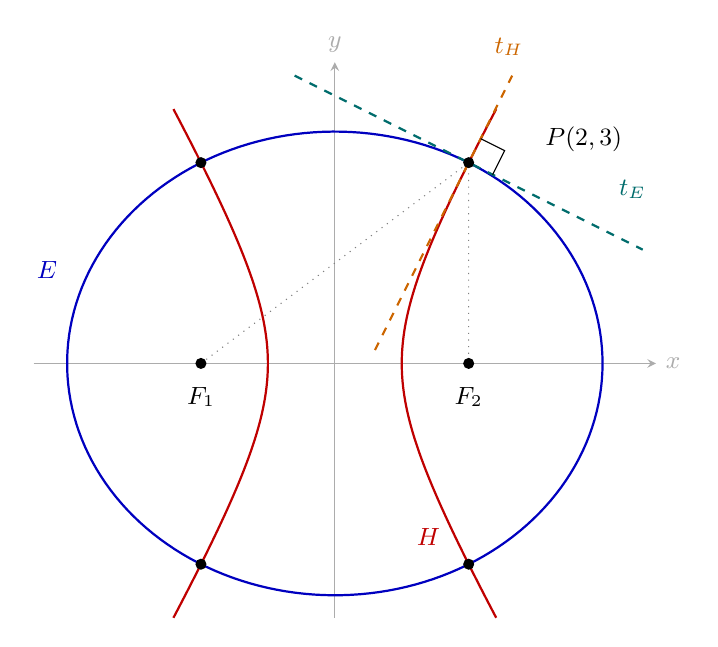
\begin{tikzpicture}[x=.85cm,y=.85cm,>=stealth,font=\small]
\draw[gray!65,->] (-4.5,0)--(4.8,0) node[right] {$x$};
\draw[gray!65,->] (0,-3.8)--(0,4.5) node[above] {$y$};
\draw[blue!75!black,thick,domain=0:360,samples=180,variable=\t]
 plot ({4*cos(\t)},{sqrt(12)*sin(\t)});
\foreach \s in {-1,1} {
\draw[red!75!black,thick,domain=-3.8:3.8,samples=100,variable=\t]
 plot ({\s*sqrt(1+\t*\t/3)},\t);}
\draw[teal!85!black,thick,dashed] (-.6,4.3)--(4.6,1.7);
\draw[orange!80!black,thick,dashed] (.6,.2)--(2.65,4.3);
\draw[gray,dotted] (-2,0)--(2,3)--(2,0);
\foreach \s in {-1,1} {\foreach \t in {-1,1}
 {\fill ({2*\s},{3*\t}) circle (2pt);}}
\fill (-2,0) circle (2pt) node[below=5pt] {$F_1$};
\fill (2,0) circle (2pt) node[below=5pt] {$F_2$};
\node[anchor=west] at (3,3.35) {$P(2,3)$};
\node[teal!85!black,anchor=west] at (4.1,2.6) {$t_E$};
\node[orange!80!black,above] at (2.6,4.45) {$t_H$};
\node[blue!75!black] at (-4.3,1.4) {$E$};
\node[red!75!black] at (1.4,-2.6) {$H$};
\draw (2.358,2.821)--(2.537,3.179)--(2.179,3.358);
\end{tikzpicture}

\end{center}

\textbf{适用条件：}
\begin{enumerate}
\item 必须是两焦点\emph{完全相同}的椭圆与双曲线，不能仅凭焦轴相同判断；
\item 两条切线必须取在\emph{同一个公共点} $P$；
\item 对所有四个公共点成立，既不依赖交点象限，也不要求焦角为特殊角。
\end{enumerate}
\end{statementbox}

\clearpage
\begin{statementbox}
\textbf{统一记号与核心参数关系（先判断共焦，再使用正交定理）。}

设椭圆、双曲线的标准方程分别为
\[
\boxed{E:\ \frac{x^2}{a^2}+\frac{y^2}{b^2}=1}\qquad
\boxed{H:\ \frac{x^2}{A^2}-\frac{y^2}{B^2}=1}.
\]
这里\textbf{小写 $a,b$ 专指椭圆}（$a>b>0$），
\textbf{大写 $A,B$ 专指双曲线}（$A,B>0$）。
也就是说，两条方程中的分母都严格大于 $0$。
两个焦点是 $F_1=(-c,0),F_2=(c,0)$，$c>0$，共焦条件是
\[
\underbrace{a^2-b^2}_{\text{椭圆焦半距平方}}
=\underbrace{A^2+B^2}_{\text{双曲线焦半距平方}}
=c^2.
\]
\begin{center}
% Two exact right triangles share the SAME segment c.
% Representative lengths: a=5,b=4,c=3,A=9/5,B=12/5.
% O=(0,0), C=(0,3), R=(4,0), Q=(-36/25,27/25).
\begin{tikzpicture}[x=1.15cm,y=1.15cm,font=\normalsize,line join=round]
\coordinate (O) at (0,0);
\coordinate (C) at (0,3);
\coordinate (R) at (4,0);
\coordinate (Q) at (-1.44,1.08);
\fill[blue!5] (O)--(R)--(C)--cycle;
\fill[red!5] (O)--(Q)--(C)--cycle;
\draw[blue!75!black,very thick] (O)--(R) node[midway,below=6pt] {$b$}
    --(C) node[midway,above right=4pt] {$a$};
\draw[red!75!black,very thick] (O)--(Q) node[midway,below left=5pt] {$A$}
    --(C) node[midway,above left=5pt] {$B$};
\draw[black,very thick] (O)--(C) node[midway,right=5pt,align=center] {$c$\\[-1pt]{\small 共用边}};
\draw[blue!75!black,thick] (0,.22)--(.22,.22)--(.22,0);
\draw[red!75!black,thick] (-1.264,.948)--(-1.132,1.124)--(-1.308,1.256);
\node[blue!75!black] at (2.25,3.65) {$a^2=b^2+c^2$};
\node[red!75!black] at (-1.6,3.65) {$c^2=A^2+B^2$};
\end{tikzpicture}

\end{center}
\textbf{看图读关系：}共用边 $c$ 是右侧三角形的直角边，
又是左侧三角形的斜边。边上标的是\emph{长度}，两次勾股定理给出
\[
a^2=b^2+\underbrace{c^2}_{A^2+B^2}
\quad\Longrightarrow\quad\boxed{a^2-A^2=b^2+B^2}.
\]
参数满足 $\boxed{a>c>A>0}$，使 $b^2=a^2-c^2>0$、$B^2=c^2-A^2>0$。
图是按参数长度构造的两个直角三角形，不是两条曲线上的焦点三角形。
在上述同中心、同坐标轴的标准式前提下，平方关系与\emph{共焦}等价；
仅有公共点并不能推出它。
\end{statementbox}
